\documentclass[letterpaper]{article} % DO NOT CHANGE THIS
\usepackage[submission]{aaai2027}  % DO NOT CHANGE THIS
\usepackage[hyphens]{url}  % DO NOT CHANGE THIS
\usepackage{graphicx} % DO NOT CHANGE THIS
\urlstyle{rm} % DO NOT CHANGE THIS
\def\UrlFont{\rm}  % DO NOT CHANGE THIS
\usepackage{natbib}  % DO NOT CHANGE THIS AND DO NOT ADD ANY OPTIONS TO IT
\usepackage{caption} % DO NOT CHANGE THIS AND DO NOT ADD ANY OPTIONS TO IT
\frenchspacing  % DO NOT CHANGE THIS
\usepackage{amsmath}
\usepackage{amssymb}
\usepackage{array}
\usepackage{algorithm}
\usepackage{algorithmicx}
\usepackage{algpseudocode}
\usepackage{booktabs}
\usepackage{multirow}

\pdfinfo{
/TemplateVersion (2027.1)
}

\setcounter{secnumdepth}{0}

\title{Adaptive Proximal Control for Federated Learning}

\author{
    Anonymous Submission
}
\affiliations{
}

\begin{document}

\maketitle

\begin{abstract}
Regularization-based federated learning methods such as FedProx and Ditto rely on a fixed proximal coefficient to regulate the coupling between client and global objectives under statistical heterogeneity. In practice, this coefficient is highly sensitive to training conditions, varies across datasets, and is typically selected through costly per-dataset tuning.

We reinterpret proximal strength as a dynamic control variable rather than a static design choice. From this perspective, we introduce AdaProx and AdaDitto, adaptive variants of FedProx and Ditto that update each client’s proximal coefficient online using a simple loss-gap signal derived from scalar quantities already exchanged during training. The proposed approach preserves the original optimization objectives and communication patterns, introduces negligible overhead, and removes the need for explicit proximal sweeps or manual tuning.

We evaluate the adaptive methods on MNIST, Fashion-MNIST, and CIFAR-100 datasets under non-IID data partitions. Across datasets, AdaProx and AdaDitto consistently recover the performance of carefully tuned static baselines while using a single shared controller configuration. On CIFAR-100, AdaDitto matches tuned Ditto (47.98\% vs. 47.72\%), and AdaProx similarly matches tuned FedProx (32.66\% vs. 32.60\%). The learned proximal coefficients evolve smoothly during training and converge to interpretable values consistent with offline tuning.

Overall, our results demonstrate that even minimal online feedback is sufficient to stabilize proximal regularization, effectively collapsing a brittle tuning dimension into an adaptive control mechanism. More broadly, this work highlights adaptive proximal control as a practical and stable alternative to fixed regularization in federated learning under heterogeneity.

\end{abstract}

\begin{links}
    \link{Code}{https://anonymous.4open.science/r/PFLlib-5B8C}
\end{links}

\section{Introduction}

Federated Learning (FL) enables collaborative training of machine learning models across distributed clients while keeping raw data local~\cite{mcmahan2017communication}. Although the underlying optimization framework is conceptually simple, practical federated systems operate under persistent heterogeneity: clients differ substantially in data distributions, availability, and local optimization dynamics. These differences—commonly referred to as statistical heterogeneity—cause local training trajectories to diverge, degrade global model quality, and lead to uneven performance across clients~\cite{mcmahan2017communication}.

Personalized Federated Learning (PFL) addresses this challenge by allowing each client to maintain a model adapted to its own data while still leveraging shared global information. Among the many approaches to FL and PFL, \emph{regularization-based} methods such as FedProx~\cite{li2020federated} and Ditto~\cite{li2021ditto} remain widely used due to their simplicity and compatibility with existing federated pipelines. These methods modify the local objective by introducing a quadratic proximal term that constrains client updates relative to a reference global model. A single scalar coefficient ($\mu$ in FedProx, $\lambda$ in Ditto) governs the strength of this constraint and mediates the trade-off between global consistency and local adaptation.

In practice, this proximal coefficient constitutes a critical point of brittleness. Prior work has shown that fixed choices of $\mu$ or $\lambda$ can be highly sensitive under heterogeneous conditions, with small changes leading to very different convergence behavior and final accuracy~\cite{yu2024effect, li2020federated, li2021ditto}. Moreover, the effective strength of proximal regularization varies across datasets and over the course of training. The standard response—manual hyperparameter tuning—is particularly ill-suited to federated settings, where partial participation, noisy evaluation signals, and high computational cost render systematic tuning expensive and unreliable~\cite{kuo2023noisy}. As a result, proximal coefficients are often chosen conservatively, sacrificing personalization to maintain stability. Throughout this paper, eliminating tuning refers to removing the need for per-dataset proximal coefficient sweeps, while using a single fixed controller configuration shared across tasks.

At a higher level, brittleness of proximal term reflects a modeling choice rather than a fundamental limitation. In control theory and optimization, algorithmic parameters are commonly interpreted as gains in a feedback system, where fixed values trade off stability and responsiveness across operating regimes. Classical results show that optimization algorithms can be viewed as feedback interconnections between systems and operators, ~\cite{lessard2016analysis}. From this perspective, treating the proximal coefficient as a fixed design constant ignores the inherent dynamics of federated training under heterogeneity.

Recent work has explored adaptivity in other aspects of federated optimization, including client-specific learning rates~\cite{kim2024adaptive}, adaptive local training schedules~\cite{shenaj2025adaptive}, dynamic regularization for drift correction~\cite{acar2021feddyn}, and variance-aware acceleration to improve convergence speed \cite{wu2023faster}. In contrast, the proximal coefficient itself—despite directly regulating the interaction between local and global objectives—remains almost universally fixed. This discrepancy points to a structural mismatch: while the degree of client drift evolves throughout training, the strength of the proximal constraint is treated as static.

In this work, we revisit proximal regularization in federated learning from a control perspective. Rather than treating the proximal coefficient as a fixed design choice, we approach it as a dynamic quantity that should respond to observed client--global misalignment. We investigate whether the brittleness associated with static proximal coefficients can be mitigated using only minimal online (during training) feedback, without modifying the underlying optimization objective or introducing additional communication overhead. The goal is not to optimize the proximal coefficient for each task, but to provide a task-independent default behavior that adapts smoothly to observed client–global misalignment during training. Here, we use \emph{brittleness} to mean undue sensitivity: small mis-specifications of the proximal coefficient can lead to disproportionately large changes in optimization stability and final performance~\cite{yu2024effect, li2020federated, li2021ditto}.

To this end, we introduce an adaptive mechanism that adjusts each client's proximal strength based on a relative loss signal: a normalized log loss-gap between the client's local loss and a server-maintained exponential moving average (EMA) of global loss. This signal is computed from scalar quantities already exchanged during training, and the resulting updates produce smooth, bounded trajectories of proximal coefficients over time.

We instantiate this mechanism as adaptive variants of FedProx and Ditto—referred to as AdaProx and AdaDitto—by wrapping the original algorithms with a client-specific controller that mediates the proximal strength via feedback. Across MNIST, Fashion-MNIST, and CIFAR-100 datasets under deliberately non-IID partitions, we evaluate whether such adaptive control can serve as a practical alternative to manually tuned proximal regularization. Our analysis shows that the resulting mechanism behaves conservatively under heterogeneity, closely matching the stability and performance of well-tuned static baselines, while the learned proximal coefficients evolve smoothly and exhibit clear, interpretable structure over training. Together, these properties indicate that minimal online feedback suffices to replace brittle, task-specific proximal tuning without additional communication overhead.


\subsection*{Contributions}

The contributions of this work are as follows:
\begin{enumerate}
    \item We reinterpret proximal regularization strength as a dynamic control variable and propose a minimal loss-gap-driven mechanism for adapting it online. We develop adaptive variants of FedProx and Ditto that integrate this mechanism without altering the underlying objectives or communication protocol.
    \item We demonstrate empirically that adaptive proximal control removes the need for per-task proximal coefficient sweeps while recovering the performance of carefully tuned static baselines using a single shared controller configuration.
\end{enumerate}

\section{Related Work}

Federated learning (FL) addresses privacy-preserving and decentralized training under client heterogeneity, where data distributions, system conditions, and optimization dynamics vary substantially across clients~\cite{mcmahan2017communication}. Regularization-based methods are particularly attractive in this setting due to their simplicity and compatibility with standard federated pipelines~\cite{li2020federated, li2021ditto}. Our work revisits this class of methods through a control-systems-oriented lens, focusing on a recurring and practically important failure mode: the brittleness of static proximal hyperparameters. High-level surveys further emphasize that sensitivity to heterogeneity, tuning burden, and system nonstationarity remain central obstacles to robust federated learning deployments~\cite{wen2023survey}.

\subsection{Static Proximal Regularization and Hyperparameter Fragility}

Regularization-based approaches mitigate client drift by constraining local updates relative to a global reference model. FedProx~\cite{li2020federated} introduces a quadratic proximal term weighted by a coefficient $\mu$ to stabilize optimization under data heterogeneity, while Ditto~\cite{li2021ditto} extends this idea to personalized models via a client-specific regularization coefficient $\lambda$. These methods are widely adopted because they preserve the underlying optimization objectives and communication protocols of federated learning.

However, their effectiveness depends critically on the choice of proximal strength. Yu et al.~\cite{yu2024effect} show that the optimal $\mu$ in FedProx varies with heterogeneity, participation rates, and training phase, and that mis-specified values can substantially degrade convergence speed and final accuracy. Similar sensitivity has been observed empirically for Ditto and related proximal methods, exposing a shared structural assumption: that a single, fixed regularization strength remains appropriate throughout federated training.

Tuning such hyperparameters in federated settings is itself challenging. Partial participation, non-IID data, and noisy evaluation signals substantially degrade the reliability of standard tuning procedures~\cite{kuo2023noisy}. Benchmarking efforts such as FedHPO-Bench highlight the high computational cost and variance associated with federated hyperparameter optimization~\cite{wang2023fedhpo}, while automated approaches such as population-based or evolutionary tuning introduce additional system complexity and overhead~\cite{guo2022auto}. Collectively, these results suggest that robustness to hyperparameter choice may be more scalable than attempting to identify precise static optima through repeated tuning.

\subsection{Adaptive and Control-Driven Federated Optimization}

Motivated by the limitations of fixed hyperparameters, recent work increasingly introduces adaptivity and feedback control into federated optimization. Several approaches frame federated learning explicitly as a dynamical system and study stability properties under adaptive update rules, providing theoretical motivation for feedback-driven design~\cite{agarwal2025adaptive}. Complementary to this perspective, feedback control has also been applied at the system level to regulate client participation and staleness, without modifying the optimization objective itself~\cite{cummins2024controlling}.

Other methods introduce adaptivity at the server aggregation stage. FedPOD employs PID-based controllers to adjust aggregation dynamics based on observed training signals, improving stability under heterogeneous data~\cite{kim2025fedpod}. Related work adapts aggregation weights using loss- or performance-based criteria to mitigate client drift and imbalance~\cite{zeng2025power}. While effective, these approaches treat client-side optimization objectives as fixed and do not modify the strength of coupling between local and global models.

A separate line of work focuses on adapting client-side training dynamics. Adaptive local training strategies adjust the number or schedule of local update steps in response to observed drift, improving robustness under non-IID data~\cite{shenaj2025adaptive}. Adaptive personalization has also been explored through client-specific model interpolation. For example, APFL learns a per-client mixing weight between global and local models to balance personalization and generalization~\cite{deng2020adaptive}. However, such approaches adapt the model combination rather than the strength of the optimization coupling itself, and still rely on fixed regularization behavior during local training. However, when combined with regularization-based personalization, such methods still rely on static proximal coefficients, implicitly assuming that the strength of client--global coupling remains appropriate throughout training.

In contrast to these approaches, our work targets a control variable that has remained largely static across prior methods: the strength of proximal coupling between local and global objectives. Rather than adapting participation, aggregation, or training schedules, we treat the proximal coefficient itself as an online control variable driven by minimal feedback. This preserves the original objectives and communication patterns of FedProx and Ditto while directly addressing a structural source of brittleness in practice.

\section{Methodology}
\label{sec:methodology}

Regularization-based baseline FL methods such as FedProx~\cite{li2020federated} and Ditto~\cite{li2021ditto} stabilize training under client heterogeneity by adding a proximal penalty to the client objective. Their performance, however, depends on a \emph{static} proximal coefficient ($\mu$ in FedProx and $\lambda$ in Ditto), whose optimal value is dataset and heterogeneity dependent and typically requires expensive hyperparameter  sweeps~\cite{yu2024effect}. We replace this fixed coefficient with an online controller that updates a client-specific coefficient each round using a loss-gap signal. This yields AdaProx and AdaDitto, which preserve the baseline algorithms except for the adaptive proximal control. The controller consists of four steps: a pre-training client loss probe, a median-EMA global loss reference, a clipped log loss-gap signal, and a smoothed bounded coefficient update. Full pseudocode is provided in the supplementary material.

\subsection{Federated setting and proximal objectives}

We consider a cross-device FL problem over clients $\mathcal{C}=\{1,\dots,N\}$. Client $i$ has data distribution $\mathcal{D}_i$ and empirical objective
$F_i(w)=\mathbb{E}_{(x,y)\sim\mathcal{D}_i}[\ell(w;x,y)]$.
At round $t$, the server broadcasts global parameters $w^{(t)}$ to a participating subset $\mathcal{S}_t$.
Each client performs $E$ local steps and returns an update for aggregation. $\arg\min_w F_i(w)$ varies across $i$, inducing client drift during local optimization.

\paragraph{FedProx and Ditto}
FedProx augments the local objective with a proximal term toward $w^{(t)}$:
\begin{equation}
\label{eq:fedprox_obj}
\min_{w}\; F_i(w) + \frac{\mu}{2}\|w-w^{(t)}\|^2.
\end{equation}
Ditto maintains a global model aggregated as in FedAvg and a personalized model $v_i$ trained via
\begin{equation}
\label{eq:ditto_obj}
\min_{v_i}\; F_i(v_i) + \frac{\lambda}{2}\|v_i-w^{(t)}\|^2,
\end{equation}
while the server aggregates only the global model updates. In both cases, the scalar coefficient governs the strength of the pull toward $w^{(t)}$ and is treated as a fixed hyperparameter in the original methods.

\subsection{Adaptive proximal control}

We define a controller that maps an observed client--global loss mismatch at round $t$ to a coefficient $\rho_i^{(t)}$ (with $\rho=\mu$ for FedProx and $\rho=\lambda$ for Ditto).

\paragraph{Per-round loss probe.}
At the start of round $t$, client $i$ evaluates the received global model $w^{(t)}$ on a small local probe minibatch $\mathcal{B}_i^{(t)}$ (drawn from its local dataset) to obtain
\begin{equation}
\label{eq:probe_loss}
\hat{L}_i^{(t)}=\frac{1}{|\mathcal{B}_i^{(t)}|}\sum_{(x,y)\in\mathcal{B}_i^{(t)}}\ell(w^{(t)};x,y).
\end{equation}
This probe is computed \emph{before} any local optimization in round $t$ so that $\hat{L}_i^{(t)}$ can capture the mismatch between the global model and client $i$'s data, rather than the effects of local training.


\paragraph{stable global loss reference.}
Each participating client also reports a scalar evaluation loss $L_i^{(t)}$ computed using the \emph{same model} $w^{(t)}$ (not the locally-updated model), to ensure comparability across clients. The server forms a stable reference via a median-EMA:
\begin{equation}
\label{eq:global_loss}
L_g^{(t)} \;=\; \beta L_g^{(t-1)} + (1-\beta)\cdot \mathrm{median}\big(\{L_i^{(t)}\}_{i\in\mathcal{S}_t}\big),
\end{equation}
where $\beta\in[0,1)$ controls smoothing. The median reduces the impact of extreme noise and temporary abnormal clients.

\paragraph{Loss-gap signal.}
We define a nonnegative, scale-robust misalignment signal as a clipped log-ratio:
\begin{equation}
\label{eq:gap}
g_i^{(t)} \;=\; \mathrm{clip}\!\left(
\log\frac{\hat{L}_i^{(t)}+\epsilon}{L_g^{(t)}+\epsilon},\; 0,\; \tau
\right),
\end{equation}
where $\epsilon>0$ avoids numerical issues and $\tau$ caps extreme ratios. By construction, $g_i^{(t)}=0$ when client $i$ is no worse than the global reference, and increases monotonically with relative underperformance.

\paragraph{Coefficient update.}
Let $\rho_i^{(t-1)}$ be client $i$'s coefficient from the previous round. We first form a target value
\begin{equation}
\label{eq:target}
\rho_i^{\ast(t)} \;=\; \rho_{\mathrm{base}} + \alpha\, g_i^{(t)},
\end{equation}
where $\rho_{\mathrm{base}}$ is a baseline proximal strength and $\alpha$ is a \emph{gain} parameter that scales how strongly the coefficient responds to the loss-gap signal $g_i^{(t)}$ (larger $\alpha$ yields more aggressive regularization increases under mismatch). To prevent abrupt round-to-round changes, we smooth the coefficient via an exponential moving average,
\begin{equation}
\label{eq:smooth}
\tilde{\rho}_i^{(t)} \;=\; (1-\gamma)\rho_i^{(t-1)} + \gamma\rho_i^{\ast(t)},
\end{equation}
where $\gamma\in(0,1]$ controls the update time-scale (smaller $\gamma$ yields slower, more stable adaptation; $\gamma=1$ removes smoothing). Finally, we enforce boundedness:
\begin{equation}
\label{eq:clip}
\rho_i^{(t)} \;=\; \mathrm{clip}(\tilde{\rho}_i^{(t)},\rho_{\min},\rho_{\max}).
\end{equation}

\subsection{Instantiations: AdaProx and AdaDitto}

\paragraph{AdaProx.}
AdaProx is obtained by replacing the static $\mu$ in \eqref{eq:fedprox_obj} with $\rho_i^{(t)}$ produced by \eqref{eq:probe_loss}--\eqref{eq:clip}:
\begin{equation}
\min_{w}\; F_i(w) + \frac{\rho_i^{(t)}}{2}\|w-w^{(t)}\|^2.
\end{equation}
All other aspects of FedProx (optimizer, local steps, and server averaging) are unchanged.

\paragraph{AdaDitto.}
Similarly, AdaDitto replaces the static $\lambda$ in \eqref{eq:ditto_obj} with $\rho_i^{(t)}$ produced by the same controller:
\begin{equation}
\min_{v_i}\; F_i(v_i) + \frac{\rho_i^{(t)}}{2}\|v_i-w^{(t)}\|^2.
\end{equation}
Global aggregation follows Ditto exactly; personalized models remain local.



\section{Experimental Setup}
\label{sec:experimental}
We evaluate whether the proposed controller (i) adapts the proximal
term in a stable manner under non-IID data and (ii) matches tuned
static baselines without performing per-dataset sweeps. In this
context, static refers to the traditional approach where proximal
coefficients ($\mu$ or $\lambda$) are treated as fixed
hyperparameters. This section describes the datasets, non-IID
partitioning, model architecture, training protocol, baselines and
reproducibility.

\subsection{Datasets}

We evaluate on three standard image-classification benchmarks commonly
used in federated and personalized federated learning.
\begin{itemize}
    \item \textbf{MNIST}~\cite{lecun2002gradient}: This dataset consists of $60,000$ training and $10,000$ test grayscale images of handwritten digits across 10 classes. In this experimental setting, it represents a low-noise, low-fragmentation environment where optimization dynamics remain comparatively stable.
    \item \textbf{Fashion-MNIST}~\cite{xiao2017fashion} : While preserving the format and scale of the original MNIST, this dataset introduces higher intra-class variability. It induces moderate heterogeneity and serves as an intermediate difficulty level between MNIST and CIFAR-100.
    \item \textbf{CIFAR-100}~\cite{krizhevsky2009learning}: This dataset contains $50,000$ training and $10,000$ testing $32 \times 32$ color images from 100 distinct classes. When subjected to label-skewed client partitions, it exhibits severe class fragmentation and serves as the primary stress-test setting for evaluating proximal regularization mechanisms.
\end{itemize}

\subsection{Non-IID Client Partitioning}
Following standard FL practice~\cite{mcmahan2017communication}, we simulate $N = 20$ clients for each
dataset under label-skewed non-IID partitions ~\cite{zhao2018federated,haller2023handling}. We specifically employ
a \textbf{pathological non-IID} setting ~\cite{mcmahan2017communication,zhang2025pfllib,zhang2022federated} where each client only holds a
small subset of the total available labels.

For MNIST and Fashion-MNIST, we enforce label-skew by restricting each
client's local dataset to samples from only 2 of the 10 classes. For
CIFAR-100, each client is assigned data from 10 of the 100 classes.

These partitions lead to a highly skewed distribution where local
models lack information about the majority of the global label space
and induce severe statistical heterogeneity and client drift. Such
settings create challenging optimization conditions where the choice
of proximal coefficient materially affects final model accuracy.

\begin{table}[tb]
\centering
\small
\setlength{\tabcolsep}{4pt}
\begin{tabular}{lccc}
\toprule
Dataset & Total & Client & Fraction \\
\midrule
MNIST & 10 & 2 & 0.20 \\
Fashion-MNIST & 10 & 2 & 0.20 \\
CIFAR-100 & 100 & 10 & 0.10 \\
\bottomrule
\end{tabular}
\caption{Label fragmentation induced by our pathological partitions (20 clients).}
\label{tab:label_frag}
\end{table}

\begin{table}[tb]
\centering
\begin{tabular}{lccc}
\toprule
Method & Parameter & Grid & Runs \\
\midrule
FedProx & $\mu$ & 3 & 3 \\
Ditto & $\lambda$ & 3 & 3 \\
\midrule
AdaProx & -- & 1 & 1 \\
AdaDitto & -- & 1 & 1 \\
\bottomrule
\end{tabular}
\caption{Proximal hyperparameter search cost for static and adaptive
  methods.}
\label{tab:hpo_cost}
\end{table}

\subsection{Baselines}

We compare our adaptive methods against the classical proximal
approaches, \textbf{FedProx}~\cite{li2020federated}, using fixed
proximal $\mu$ and \textbf{Ditto}~\cite{li2021ditto}, using fixed
personalization weight $\lambda$.

For each dataset, FedProx and Ditto are evaluated using a two-stage
tuning procedure. We first identify a coarse operating range for the
proximal coefficient ($\mu$ or $\lambda$) using a representative grid
($\{0.05, 0.20, 1.00\}$), reflecting common tuning practices in
federated settings. In this context, a grid size of 3 (as shown in
Table~\ref{tab:hpo_cost}) indicates that for the static baselines, the
training process must be repeated three separate times—once for each
entry in the grid—to determine which setting performs best. Within
this range, a small local refinement is done by performing further
lightweight tests on a smaller subset of the data, to select a stable
per-dataset operating point, and we report the best-performing static
configuration.
This refinement uses short diagnostic runs on a reduced budget and
does not count as an additional full training run in
Table~\ref{tab:hpo_cost}.
This procedure mirrors realistic tuning budgets under noisy federated
evaluation and serves as the reference against which adaptive control
is compared.

Table~\ref{tab:hpo_cost} reports the proximal hyperparameter search
cost for both static and adaptive approaches. Static baselines need
several full training runs per dataset to tune $\mu$ or $\lambda$,
whereas adaptive methods rely on a single controller configuration
reused across all experiments.

\begin{table}[tb]
\centering
\begin{tabular}{lccccccc}
\toprule
$\mu_{\text{base}}$ & $\mu_{\min}$ & $\mu_{\max}$ & $\alpha$ & $\tau$
  & $\gamma$ & $\beta$ & $\epsilon$\\
\midrule
0.08 & 0.05 & 3.0 & 0.8 & 0.7 & 0.3 & 0.9 & 0.0001\\
\bottomrule
\end{tabular}
\caption{Controller hyperparameters used for AdaProx and AdaDitto for
  all datasets.}
\label{tab:controller-hparams}
\end{table}

\begin{table*}[t]
  \centering
  \small
  \setlength{\tabcolsep}{5pt}
  \begin{tabular}{llcccc}
    \toprule
    Dataset & Method & Global Acc. & Pers. Acc. & Alg. time/run (s) & Seq. tuning budget (s) \\
    \midrule
    \multirow{2}{*}{MNIST}
      & FedProx  & 0.9774 & ---    & 3590.6  & 10771.8 \\
      & AdaProx  & 0.9781 & ---    & 3841.9  & \textbf{3841.9} \\
    \addlinespace
      & Ditto    & 0.9921 & 0.9919 & 5911.5  & 17734.5 \\
      & AdaDitto & 0.9923 & 0.9921 & 6325.3  & \textbf{6325.3} \\
    \midrule
    \multirow{2}{*}{FMNIST}
      & FedProx  & 0.8475 & ---    & 3412.2  & 10236.7 \\
      & AdaProx  & 0.8449 & ---    & 3651.1  & \textbf{3651.1} \\
    \addlinespace
      & Ditto    & 0.9740 & 0.9727 & 5576.2  & 16728.6 \\
      & AdaDitto & 0.9729 & 0.9719 & 5966.5  & \textbf{5966.5} \\
    \midrule
    \multirow{2}{*}{CIFAR-100}
      & FedProx  & 0.3260 & ---    & 3374.9  & 10124.7 \\
      & AdaProx  & 0.3266 & ---    & 3611.1  & \textbf{3611.1} \\
    \addlinespace
      & Ditto    & 0.4772 & 0.4721 & 6745.3  & 20235.9 \\
      & AdaDitto & 0.4798 & 0.4741 & 7217.5  & \textbf{7217.5} \\
    \bottomrule
  \end{tabular}
  \caption{Mean test accuracies and \textbf{algorithmic training cost}. FedProx and AdaProx do not have personalized accuracy.
  \emph{Algorithmic time/run} measures the runtime required by the
  learning algorithm itself (local training, aggregation, and adaptive
  control), excluding analysis-only instrumentation.
  \emph{Sequential tuning budget} reports an accounting estimate
  assuming sequential evaluation of three candidate proximal
  coefficients for static methods and a single run for adaptive
  methods; this reflects tuning burden rather than wall-clock
  performance.}
  \label{tab:overall-acc-alg}
\end{table*}



\subsection{Controller hyperparameters (fixed, untuned)}

All controller hyperparameters in Table~\ref{tab:controller-hparams}
are selected once and then reused \emph{unchanged} across all datasets
and experiments. We choose a single conservative configuration using
simple heuristics and a small number of pilot runs whose sole purpose
was to ensure stable training (i.e., no divergence or oscillatory
coefficient behavior). Crucially, we do \emph{not} perform any
dataset-specific tuning or search over these values.
These pilots were used only as a safety check for stability (no
divergence), not to optimize accuracy on any dataset.
This is done to show that adaptive proximal control can remove the
need for per-dataset proximal sweeps by providing a single set of
task-independent defaults.



\subsection{Models and Training Configuration}

To isolate the influence of optimization and proximal control, all
methods use the same backbone: a lightweight four-layer convolutional
neural network (CNN), identical across datasets and trained from
scratch for each experiment.

All experiments follow the same federated training protocol: 200
global rounds with full client participation (20/20 clients per
round). Clients optimize locally using SGD with a fixed learning rate
$\eta = 0.005$ for one local epoch per round, using 10 minibatches
per epoch. These choices are held constant to isolate the effect of
proximal control under identical optimization and communication
conditions.
\subsection{Performance Metrics}

\paragraph{\textbf{Accuracy}:} We report \textit{Global accuracy}, which is the test accuracy of the aggregated global model on the standard test set. For Ditto-style methods, we additionally report \textit{personalized accuracy}, computed by evaluating each client's personalized model on its local test split and averaging across clients.

\paragraph{\textbf{Algorithmic time/run}:} \textit{Algorithmic time/run} estimates the compute required by the learning algorithm itself (local training, aggregation, and controller-required probe loss), excluding analysis-only instrumentation such as probe accuracy evaluation, extensive logging, and diagnostic sampling; see the supplementary runtime analysis.

\paragraph{\textbf{Sequential tuning budget}:} Static proximal methods are typically run multiple times to select $\mu$ or $\lambda$. To reflect this tuning burden, we report a \textit{sequential tuning budget} computed as:
\[
    T_{\text{budget}} = (\text{\# full training runs}) \times T_{\text{alg}}.
\]
For static methods the number of runs required is three per dataset, one for each candidate proximal term; the adaptive methods only require a single run per dataset. This metric isolates the practical cost of hyperparameter brittleness rather than raw per-run speed.





\subsection{Implementation and Reproducibility}
All experiments are implemented in PyTorch by extending the
\textbf{PFLlib}~\cite{zhang2025pfllib} library containing standardized
implementations of FedProx, Ditto, and other FL algorithms. We
implement AdaProx and AdaDitto as wrappers around the existing FedProx
and Ditto modules, enabling direct comparisons under identical
pipelines.

To ensure the reproducibility of our results, we use a fixed random
seed of 42 for PyTorch, NumPy, and dataset shuffling. All experiments
were conducted on a system equipped with an NVIDIA GeForce RTX 3060 Ti
(8 GB RAM). However, because CIFAR-100 experiments use GPU kernels
with nondeterministic operations (e.g., certain CuDNN backends), minor
run-to-run variation is expected. The anonymous code link is provided in the links block after the abstract.

\begin{figure*}[t]
  \centering
  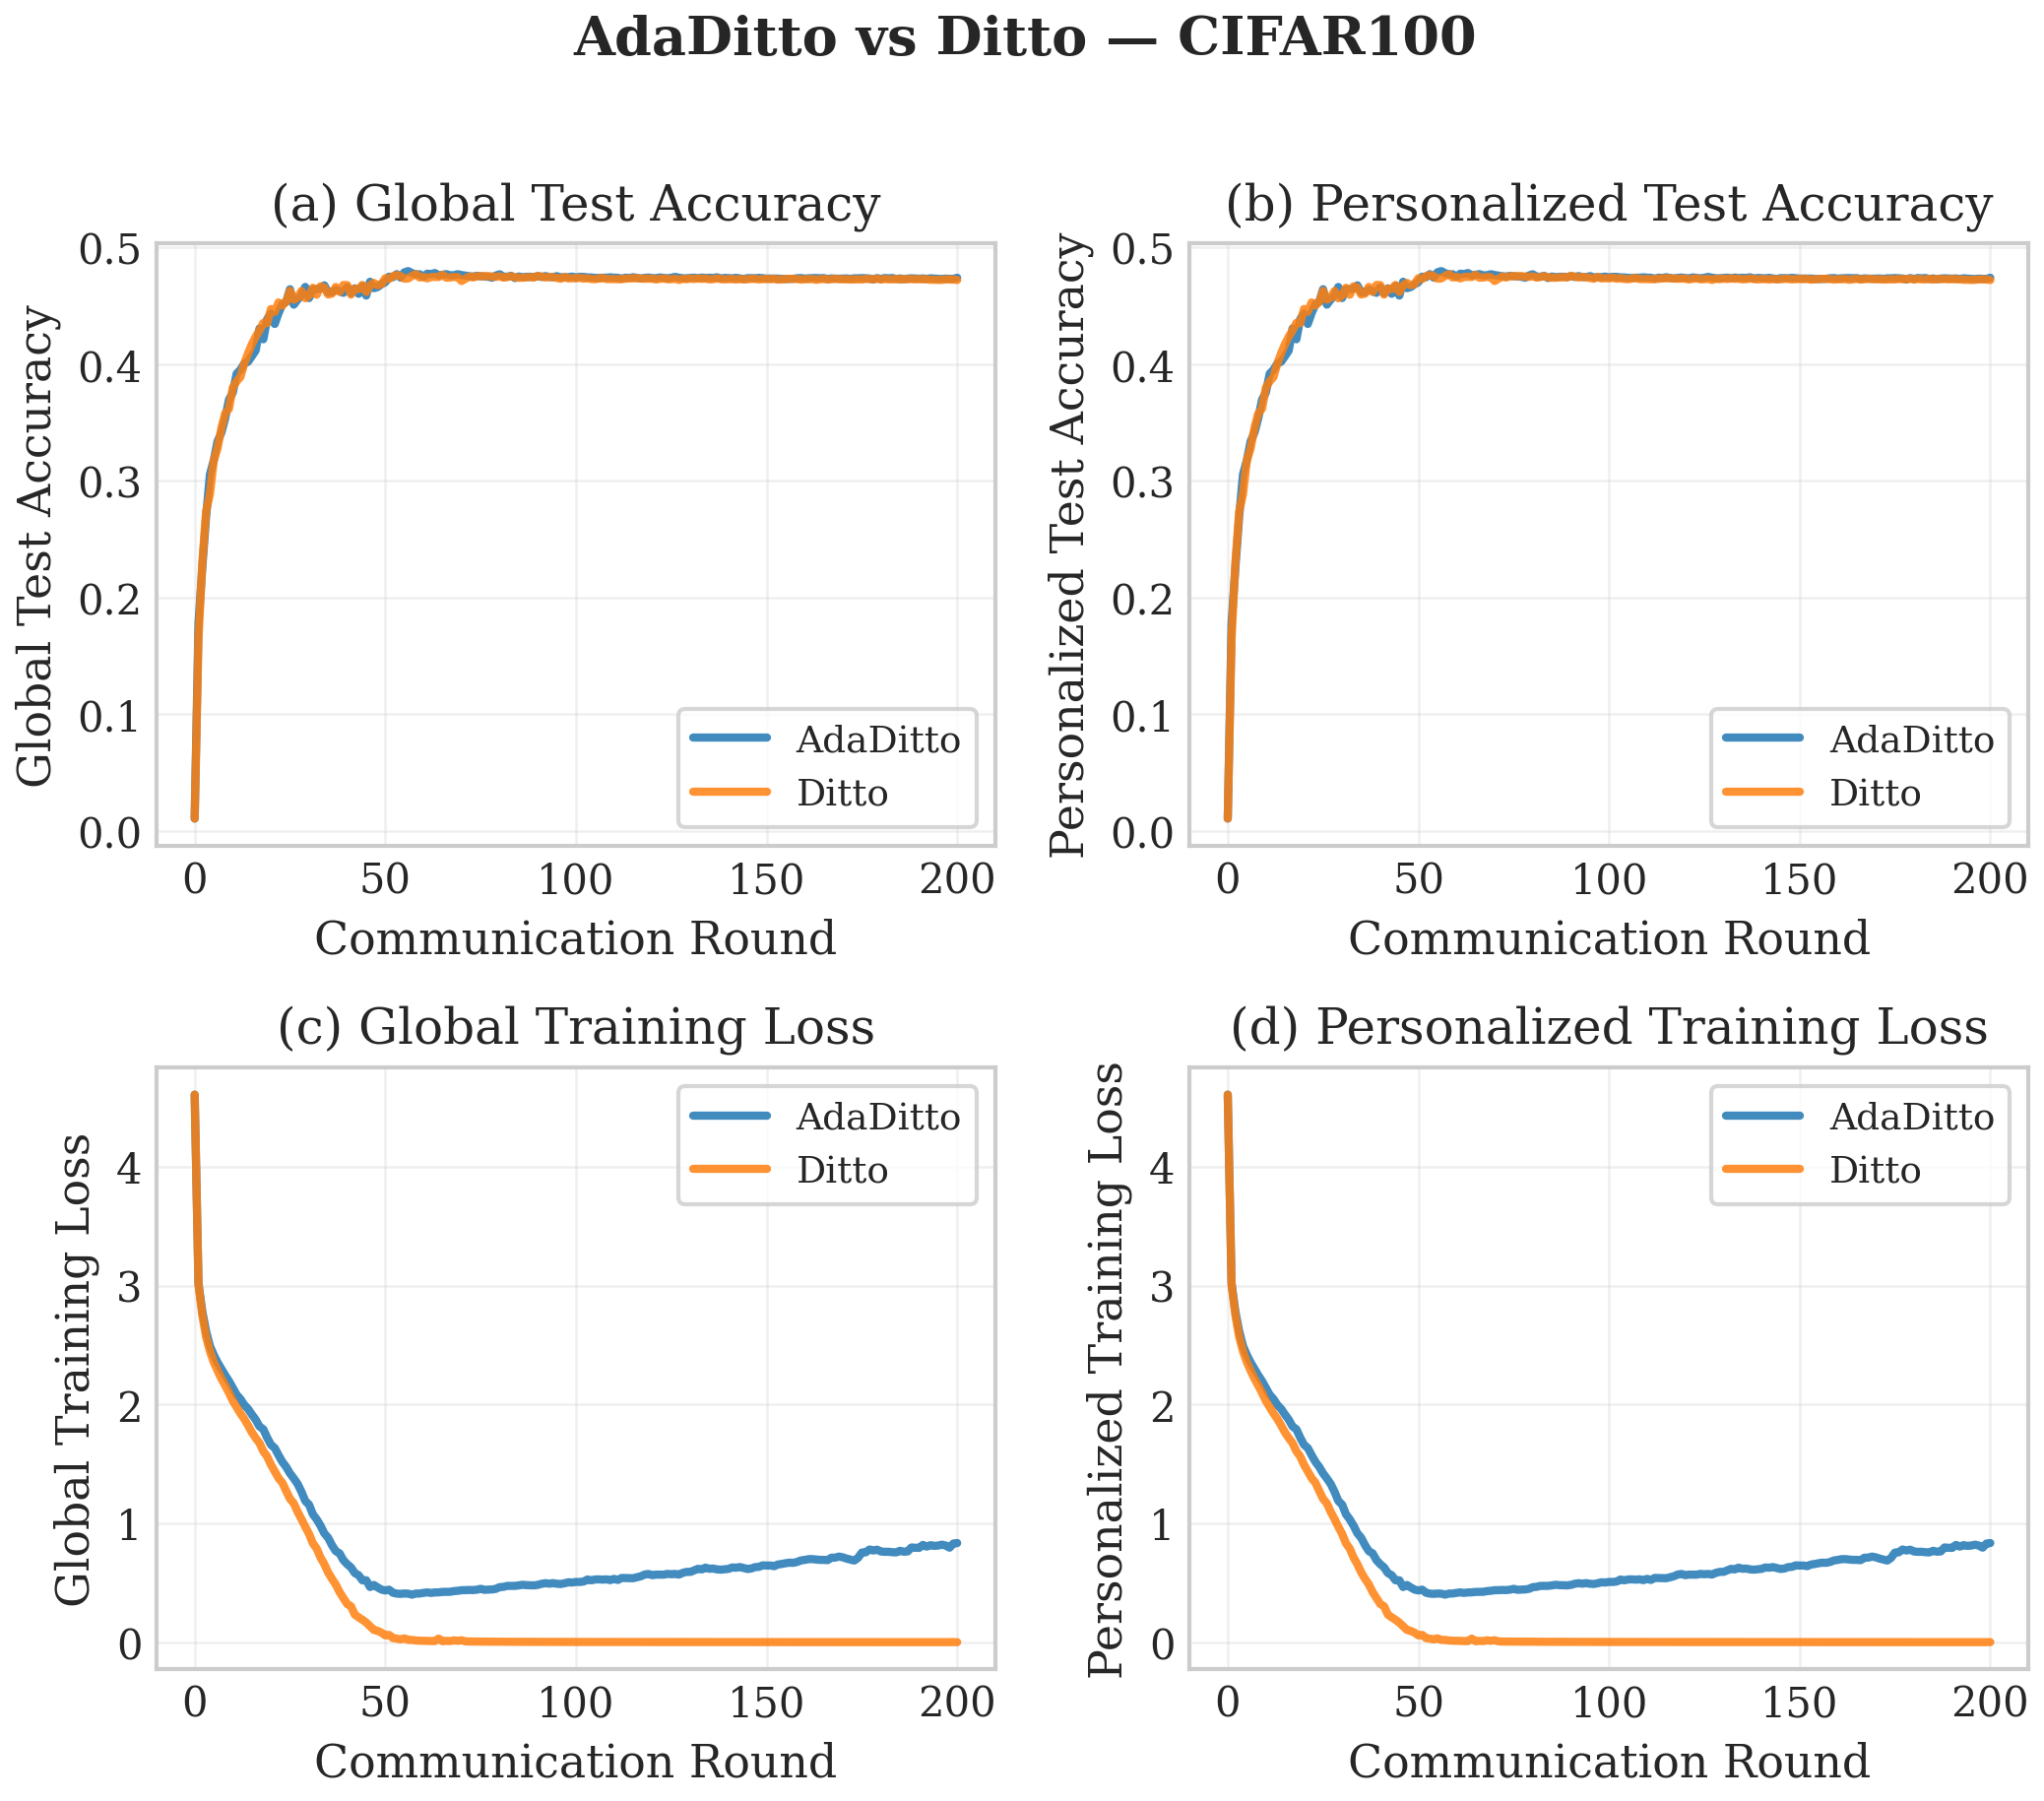
\includegraphics[width=0.8\textwidth]{Figures/cifar100_adaditto_vs_ditto.png}
  \caption{CIFAR-100: AdaDitto vs.\ Ditto — global and personalized
    accuracy and training loss. AdaDitto maintains
    higher training loss due to stronger learned regularization while
    recovering Ditto's tuned accuracy.}
  \label{fig:cifar-adaditto}
\end{figure*}



\section{Results}
\label{sec:results}

We evaluate AdaProx and AdaDitto on MNIST, Fashion-MNIST, and
CIFAR-100 under the non-IID settings described in
the experimental setup. Our primary analysis focuses on
CIFAR-100, the most heterogeneous and fragmented setting. Results for
MNIST and Fashion-MNIST show similar patterns and are included in
the supplementary additional results, with a brief synopsis
provided here.

Our analysis addresses two questions:
(i) Does the adaptive mechanism behave conservatively under
heterogeneity?
(ii) What structure emerges in the learned proximal coefficients over
training?

\subsection{Overall Accuracy and Single-Run Training Cost}

Table~\ref{tab:overall-acc-alg} reports mean test accuracy, algorithmic
training time per run, and the corresponding sequential tuning budget.
FedProx and Ditto use their best static proximal coefficients selected
offline, while AdaProx and AdaDitto use a single fixed controller
configuration shared across all datasets.



\paragraph{Key observation.}
Adaptive methods incur a small algorithmic per-run overhead relative
to static baselines, but operate under a fixed single-run training
budget. In contrast, static methods require multiple full training
runs to identify suitable proximal coefficients. As shown in
Table~\ref{tab:overall-acc-alg}, adaptive methods consistently achieve
comparable accuracy while substantially reducing the total sequential
tuning budget—by up to 71\% for AdaDitto over Ditto on MNIST.
A detailed runtime decomposition and algorithmic overhead
quantification are provided in the supplementary runtime analysis.





\begin{figure}[tb]
  \centering
  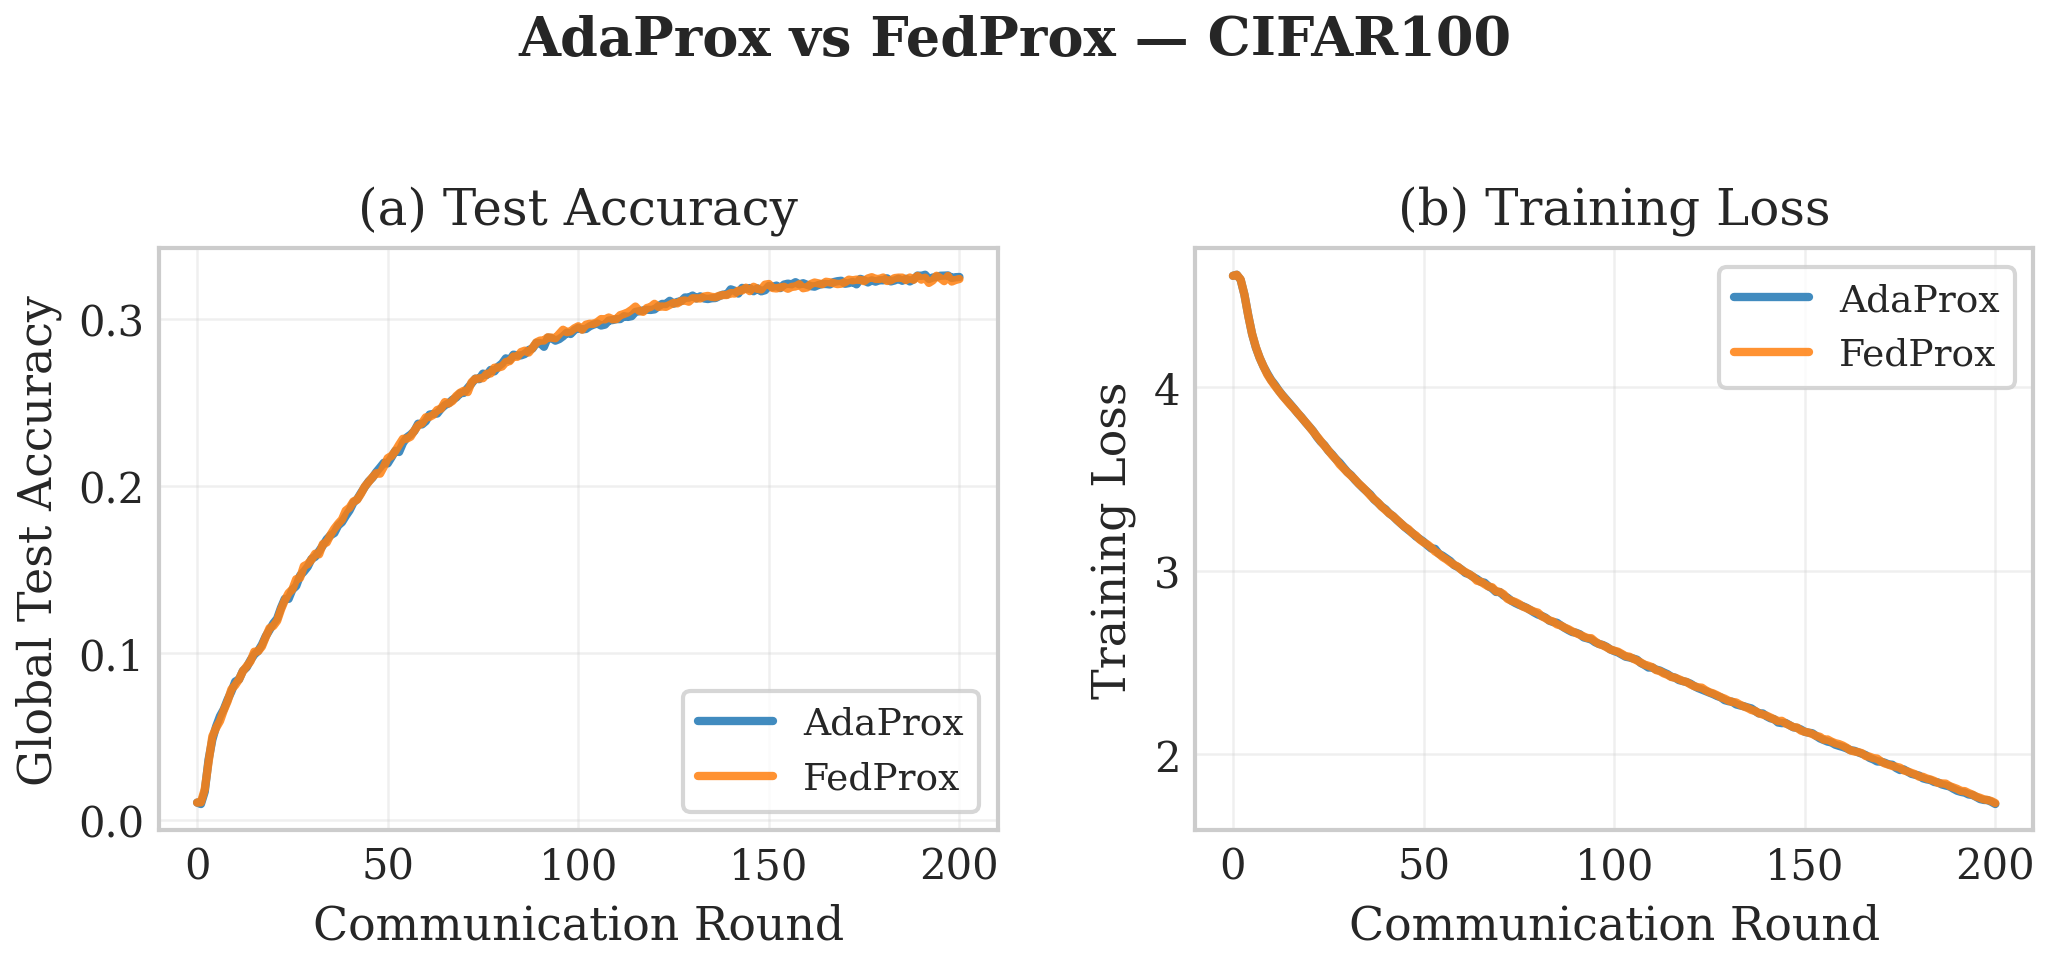
\includegraphics[width=\columnwidth]{Figures/cifar100_adaprox_vs_fedprox.png}
  \caption{CIFAR-100: AdaProx vs.\ FedProx --- global test accuracy
  and training loss. The tuned FedProx baseline corresponds to
  $\mu = 0.08$. AdaProx learns a small non-zero proximal strength
  while matching performance.}
  \label{fig:cifar-adaprox}
\end{figure}

\begin{figure}[tb]
  \centering
  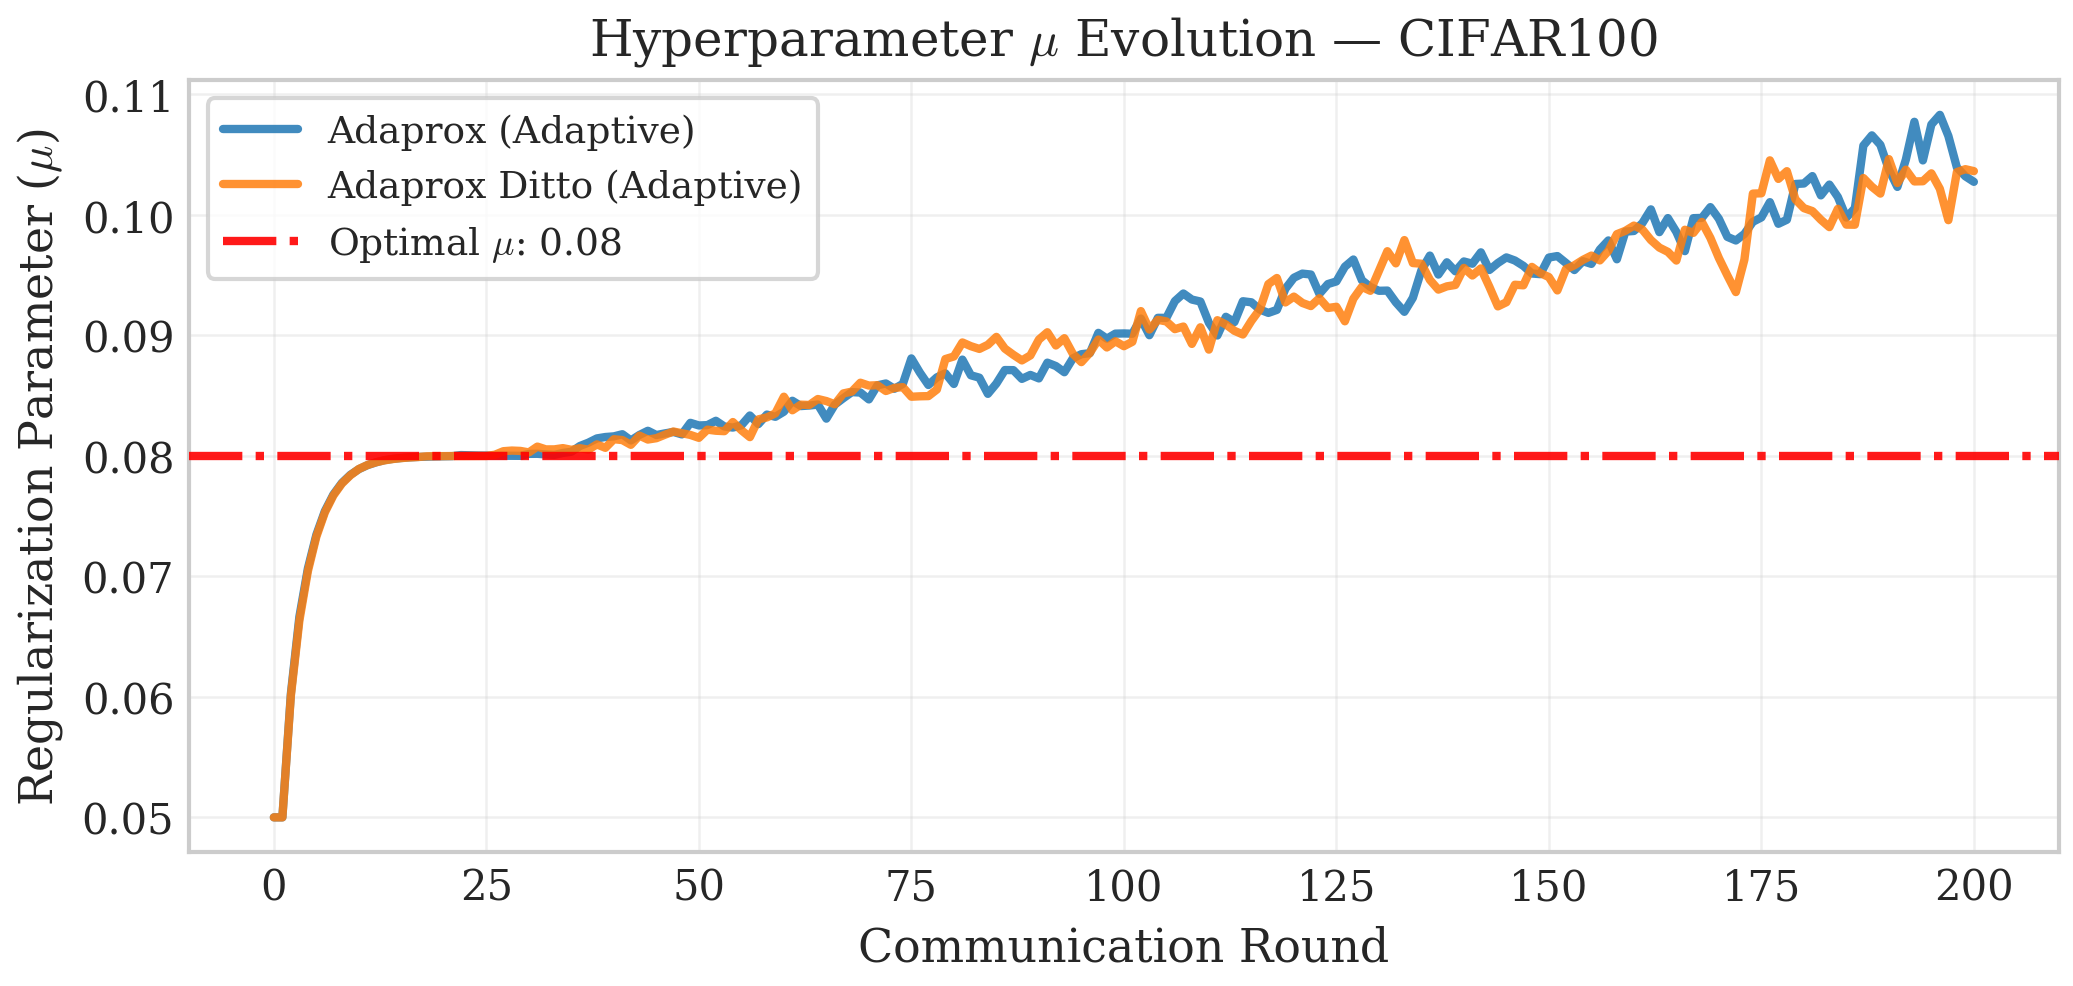
\includegraphics[width=\columnwidth]{Figures/cifar100_mu_evolution.png}
  \caption{CIFAR-100: evolution of the learned proximal coefficient
  for AdaProx and AdaDitto. Both methods rapidly increase $\mu$
  toward the tuned operating region and continue adapting smoothly
  as heterogeneity persists.}
  \label{fig:cifar-evolution}
\end{figure}

\subsection{CIFAR-100: Adaptive vs.\ Static Personalization}

Figures~\ref{fig:cifar-adaditto}--\ref{fig:cifar-evolution} compare
adaptive and static proximal methods under CIFAR-100 conditions.
\noindent \paragraph{Accuracy:}
Adaptive proximal control matches tuned static baselines. AdaDitto
reaches essentially the same final accuracy as Ditto (within
$\pm 0.002$). AdaProx likewise tracks tuned FedProx throughout
training.

\paragraph{Loss behaviour:}
Similar accuracy can hide different dynamics. Ditto keeps pushing
training loss toward zero, while AdaDitto settles earlier at a higher
loss but the same accuracy, indicating stronger regularization under
mismatch. For FedProx, AdaProx and tuned FedProx have almost identical
loss curves, suggesting the controller remains mild and stable.

\subsection{Evolution of the Learned Proximal Coefficient}

Figure~\ref{fig:cifar-evolution} plots the learned proximal coefficient
$\mu$ over rounds on CIFAR-100. Early on, $\mu$ increases quickly from
its initial value (0.05) to 0.08, meaning the controller rapidly
strengthens the proximal pull when the global model is most mismatched
to clients. In mid training, $\mu$ stays close to 0.08 with small
oscillations, showing that the adaptive rule settles near the same
value found by offline tuning. Late in training, $\mu$ rises slowly
toward 0.10–0.11, indicating that heterogeneity persists near
convergence and the controller responds by increasing regularization
rather than letting it decay.

This shows that the controller rapidly converges to the tuned operating point in this setting and then keeps adjusting smoothly as non-IID effects remain, which explains why the adaptive methods track tuned static baselines while keeping $\mu$ stable and interpretable throughout.

\subsection{Behaviour on MNIST and Fashion-MNIST}

Results for MNIST and Fashion-MNIST demonstrate that adaptive proximal
control remains stable and non-degrading in settings with lower
heterogeneity. As detailed in the supplementary additional results,
accuracy curves for AdaProx and AdaDitto overlap almost exactly with
their optimally tuned static counterparts, reaching saturation near
baseline performance.
Notably, AdaDitto consistently maintains a higher training loss; this
indicates that the controller successfully prioritizes global
generalization over local overfitting, even when the data is easily
learnable.


\paragraph{Limitations.}
Our experiments use full participation, lightweight CNNs, and controlled label-skewed partitions. Evaluating adaptive proximal control under partial participation, device churn, larger architectures, and language or multimodal tasks remains future work.

\section{Conclusion}
We reinterpret proximal regularization in federated learning as a control problem and show that even minimal online feedback can replace brittle, per-dataset proximal sweeps with a stable adaptive mechanism. AdaProx and AdaDitto update proximal strength online using a simple client--global loss gap, replacing brittle offline sweeps with an interpretable feedback mechanism that responds directly to misalignment.

Across the heterogeneous settings studied, the adaptive methods match tuned FedProx and Ditto while using a single controller configuration. Broadly, parameters that trade off global consistency against local adaptation need not be fixed design constants; they can be treated as adaptive state variables driven by training dynamics.


\bibliography{references}
% \input{ReproducibilityChecklist.tex}

\end{document}
